% !TEX root = ../main.tex

\chapter{计算方法大作业:}
\begin{center}
    \textbf{用不同数值方法计算积分$\int_{0}^{1} \sqrt{x} \ln x  \ dx = -\frac{4}{9}$}
\end{center}

\section*{1. 利用复化梯形公式和复化辛普森公式计算积分}

取不同的步长 $h$,分别用复化梯形公式和复化辛普森公式计算积分,给出误差中关于$h$的函数,并与积分精确值比较两个公式的精度,是否存在一个最小的$h$,使得精度不能再被改善?

本问题可以分解为三个子问题:
\begin{enumerate}
    \item 利用复化梯形公式求解给定积分问题,并给出误差中关于$h$的函数。
    \item 利用复化辛普森公式求解给定积分问题,并给出误差中关于$h$的函数。
    \item 与积分精确值比较复化梯形公式和复化辛普森公式的精度。
    \item 探究:是否存在一个最小的$h$,使得精度不能再被改善?
\end{enumerate}

根据以上分类,我们用以下四小节来分别解答这四个问题。

\subsection*{1.1 利用复化梯形公式求解给定积分问题,并给出误差中关于$h$的函数}

令$f(x) = \sqrt{x} \ln x$,设将区间$[a,b]$划分为$n$等份,等分点$x_k = a + kh$,$h = \frac{b-a}{n},k=0,1,2,3,...,n$。由此得到复化梯形公式:
\begin{equation}
    T_n = \frac{h}{2} [f(a) + 2\sum_{k=1}^{n-1} f(x_k) + f(b) ]
    \label{eq:compound_trapezoid_general}
\end{equation}
复合梯形公式的余项为:
\begin{equation}
    R_n(f) = -\frac{b-a}{12} h^2 f^{\prime\prime} (\eta), \\ \eta\in(0,1)
    \label{eq:compound_trapezoid_R_general}
\end{equation}

在本题中,$a=0,b=1$,且因为$f(0) \rightarrow -\infty$,我们这里令$f(0) = \lim_{x \rightarrow 0} \sqrt{x} \ln x$,同时$f(1) = 0$。等分点$x_k$也可以写作:$x_k = kh$,其中$h = \frac{1}{n},k=0,1,2,3,...,n$。根据以上分析,$f(x)$的复化梯形公式可以写为:
\begin{equation}
    T_n = \frac{h}{2} \left(\lim_{x\rightarrow 0} \sqrt{x} \ln x + 2 \sum_{k=1}^{n-1} \sqrt{kh} \ln(kh)\right)
    \label{eq:compound_trapezoid_f}
\end{equation}
计算$f(x)$的各阶导数:
\begin{equation}
    \begin{aligned}
        f^{(1)}(x) & = \frac{1}{2} x^{-\frac{1}{2}} (\ln x + 2) \\
        f^{(2)}(x) & = -\frac{1}{4} x^{-\frac{3}{2}} \ln x \\
        f^{(3)}(x) & = \frac{1}{4} x^{-\frac{5}{2}} (\frac{3}{2} \ln x -1) \\
        f^{(4)}(x) & = x^{-\frac{7}{2}} - \frac{15}{16} x^{-\frac{7}{2}} \ln x
    \end{aligned}
    \label{eq:f_diff}
\end{equation}

将上式带入公式(\ref{eq:compound_trapezoid_R_general})中,得到$f(x)$复化梯形公式的误差函数:
\begin{equation}
    R_n(f) = \frac{h^2}{48} \eta^{-\frac{3}{2}} \ln \eta
    \label{eq:compound_trapezoid_R_f}
\end{equation}

\subsection*{1.2 利用复化辛普森公式求解给定积分问题,并给出误差中关于$h$的函数}

若记$x_{k+1/2} = x_k + \frac{1}{2}h$,则得到复化辛普森公式为:
\begin{equation}
    \begin{aligned}
        S_n & = \frac{h}{6} \sum_{k=0}^{n-1} [f(x_k) + 4f(x_{k+1/2}) + f(x_{k+1})] \\
            & = \frac{h}{6} [f(a) + 4\sum_{k=0}^{n-1} f(x_{k+1/2}) + 2\sum_{k=1}^{n-1} f(x_{k}) + f(b)]
    \end{aligned}
    \label{eq:Simpson_general}
\end{equation}
当$f(x) \in \mathcal{C}^4[a,b]$时,复化辛普森公式的余项为:
\begin{equation}
    R_n(f) = - \frac{b-a}{180} \left(\frac{h}{2}\right) f^{(4)}(\eta), \\ \eta \in (a,b)
    \label{eq:simpson_diff}
\end{equation}

在本题中,$a=0,b=1$,且因为$f(0) \rightarrow -\infty$,我们这里令$f(0) = \lim_{x \rightarrow 0} \sqrt{x} \ln x$,同时$f(1) = 0$。等分点$x_k$也可以写作:$x_k = kh$,其中$h = \frac{1}{n},k=0,1,2,3,...,n$。根据以上分析,$f(x)$的复化辛普森公式可以写为:
\begin{equation}
    S_n = \frac{h}{6} \left(\lim_{x\rightarrow 0} \sqrt{x} \ln x + 4 \sum_{k=0}^{n-1} \sqrt{\frac{(2k+1)h}{2}} \ln \frac{(2k+1)h}{2} + 2\sum_{k=1}^{n-1} \sqrt{kh} \ln (kh)\right)
    \label{eq:compound_simpson_f}
\end{equation}

将$f(x)$的导数结果(\ref{eq:f_diff})带入公式(\ref{eq:simpson_diff})中,得到$f(x)$复化辛普森公式的误差函数:
\begin{equation}
    R_n(f) = \frac{h^4}{2880} \eta^{-\frac{7}{2}} (\frac{15}{16} \ln \eta - 1)
    \label{eq:compound_simpson_R_f}
\end{equation}

\subsection*{1.3 与积分精确值比较复化梯形公式和复化辛普森公式的精度}

取区间等分份数$n$为2的指数倍,进行仿真,得到复化梯形公式和复化辛普森公式的精度对比表如下:
\begin{table}[!hpt]
    \caption[梯形和辛普森求积结果对比]{复化梯形公式和复化辛普森公式的精度比较表\\(精确值$\int_{0}^{1} \sqrt{x} \ln x  \ dx = -\frac{4}{9}=-0.444444\cdots$)}
    \label{tab:tb_t_simpson}
    \centering
    \begin{tabular}{@{}cccccc@{}} \toprule
                      &         & \multicolumn{2}{c}{复化梯形公式} & \multicolumn{2}{c}{复化辛普森公式} \\ \cmidrule(r){3-4} \cmidrule(r){5-6}
        区间等分份数$n$ & 步长 $h$                   & 求积结果             & 误差                           & 求积结果 & 误差                    \\ \midrule
        1             & 1                         & $-6.90775\times10^{-9}$ & 0.444444  & -0.326752 & 0.117691 \\
        2             & 0.5                       & -0.245064 & 0.199379                & -0.395783 & 0.048660 \\
        4             & 0.25                      & -0.358104 & 0.086340                & -0.424752 & 0.019692 \\
        8             & 0.125                     & -0.408090 & 0.036354                & -0.436602 & $7.841677\times10^{-3}$\\
        16            & $6.25\times 10^{-2}$      & -0.429474 & 0.014969                & -0.441361 & $3.083324\times10^{-3}$\\
        32            & $3.125\times 10^{-2}$     & -0.438389 & $6.054958\times10^{-3}$ & -0.443244 & $1.200028\times10^{-3}$\\
        64            & $1.5625\times 10^{-2}$    & -0.442030 & $2.413760\times10^{-3}$ & -0.443981 & $4.631324\times10^{-4}$\\
        128           & $7.8125\times 10^{-3}$    & -0.443493 & $9.507894\times10^{-4}$ & -0.444266 & $1.774805\times10^{-4}$\\
        256           & $3.90625\times 10^{-3}$   & -0.444073 & $3.708077\times10^{-4}$ & -0.444376 & $6.760613\times10^{-5}$\\
        512           & $1.953125\times 10^{-3}$  & -0.444301 & $1.434065\times10^{-4}$ & -0.444418 & $2.561969\times10^{-5}$\\
        1024          & $9.765625\times 10^{-4}$  & -0.444389 & $5.506639\times10^{-5}$ & -0.444434 & $9.665089\times10^{-6}$\\
        % 2048          & $4.8828125\times 10^{-4}$ & -0.444423 & $2.101541\times10^{-5}$ & -0.444440 & $3.631789\times10^{-6}$\\
\bottomrule
    \end{tabular}
  \end{table}
%   1             & 1                         & $-6.90775527898214\times10^{-9}$ & 0.444444437536689 & -0.326752715257044 & 0.117691729187400 \\
%   2             & 0.5                       & -0.245064539321014 & 0.199379905123430               & -0.395783900178324 & 0.0486605442661203 \\
%   4             & 0.25                      & -0.358104060539643 & 0.0863403839048014              & -0.424752033280332 & 0.0196924111641126 \\
%   8             & 0.125                     & -0.408090040382983 & 0.0363544040614617              & -0.436602766716599 & $7.84167772784578\times10^{-3}$\\
%   16            & $6.25\times 10^{-2}$      & -0.429474585277106 & 0.0149698591673382              & -0.441361119859201 & $3.08332458524363\times10^{-3}$\\
%   32            & $3.125\times 10^{-2}$     & -0.438389486285633 & $6.05495815881146\times10^{-3}$ & -0.443244416215240 & $1.20002822920440\times10^{-3}$\\
%   64            & $1.5625\times 10^{-2}$    & -0.442030683768816 & $2.41376067562826\times10^{-3}$ & -0.443981312032037 & $4.63132412407308\times10^{-4}$\\
%   128           & $7.8125\times 10^{-3}$    & -0.443493654984221 & $9.50789460223589\times10^{-4}$ & -0.444266963911217 & $1.77480533227581\times10^{-4}$\\
%   256           & $3.90625\times 10^{-3}$   & -0.444073636688462 & $3.70807755982083\times10^{-4}$ & -0.444376838308117 & $6.76061363274472\times10^{-5}$\\
%   512           & $1.953125\times 10^{-3}$  & -0.444301037907701 & $1.43406536743884\times10^{-4}$ & -0.444418824753807 & $2.56196906375239\times10^{-5}$\\
%   1024          & $9.765625\times 10^{-4}$  & -0.444389378044529 & $5.50663999154821\times10^{-5}$ & -0.444434779354570 & $9.66508987476633\times10^{-6}$\\
%   2048          & $4.8828125\times 10^{-4}$ & -0.444423429028184 & $2.10154162605947\times10^{-5}$ & -0.444440812655215 & $3.63178922924146\times10^{-6}$\\

为了更形象对比两种方法的误差,上表可以可视化为下图:
\begin{figure}[!htp]
    \centering
    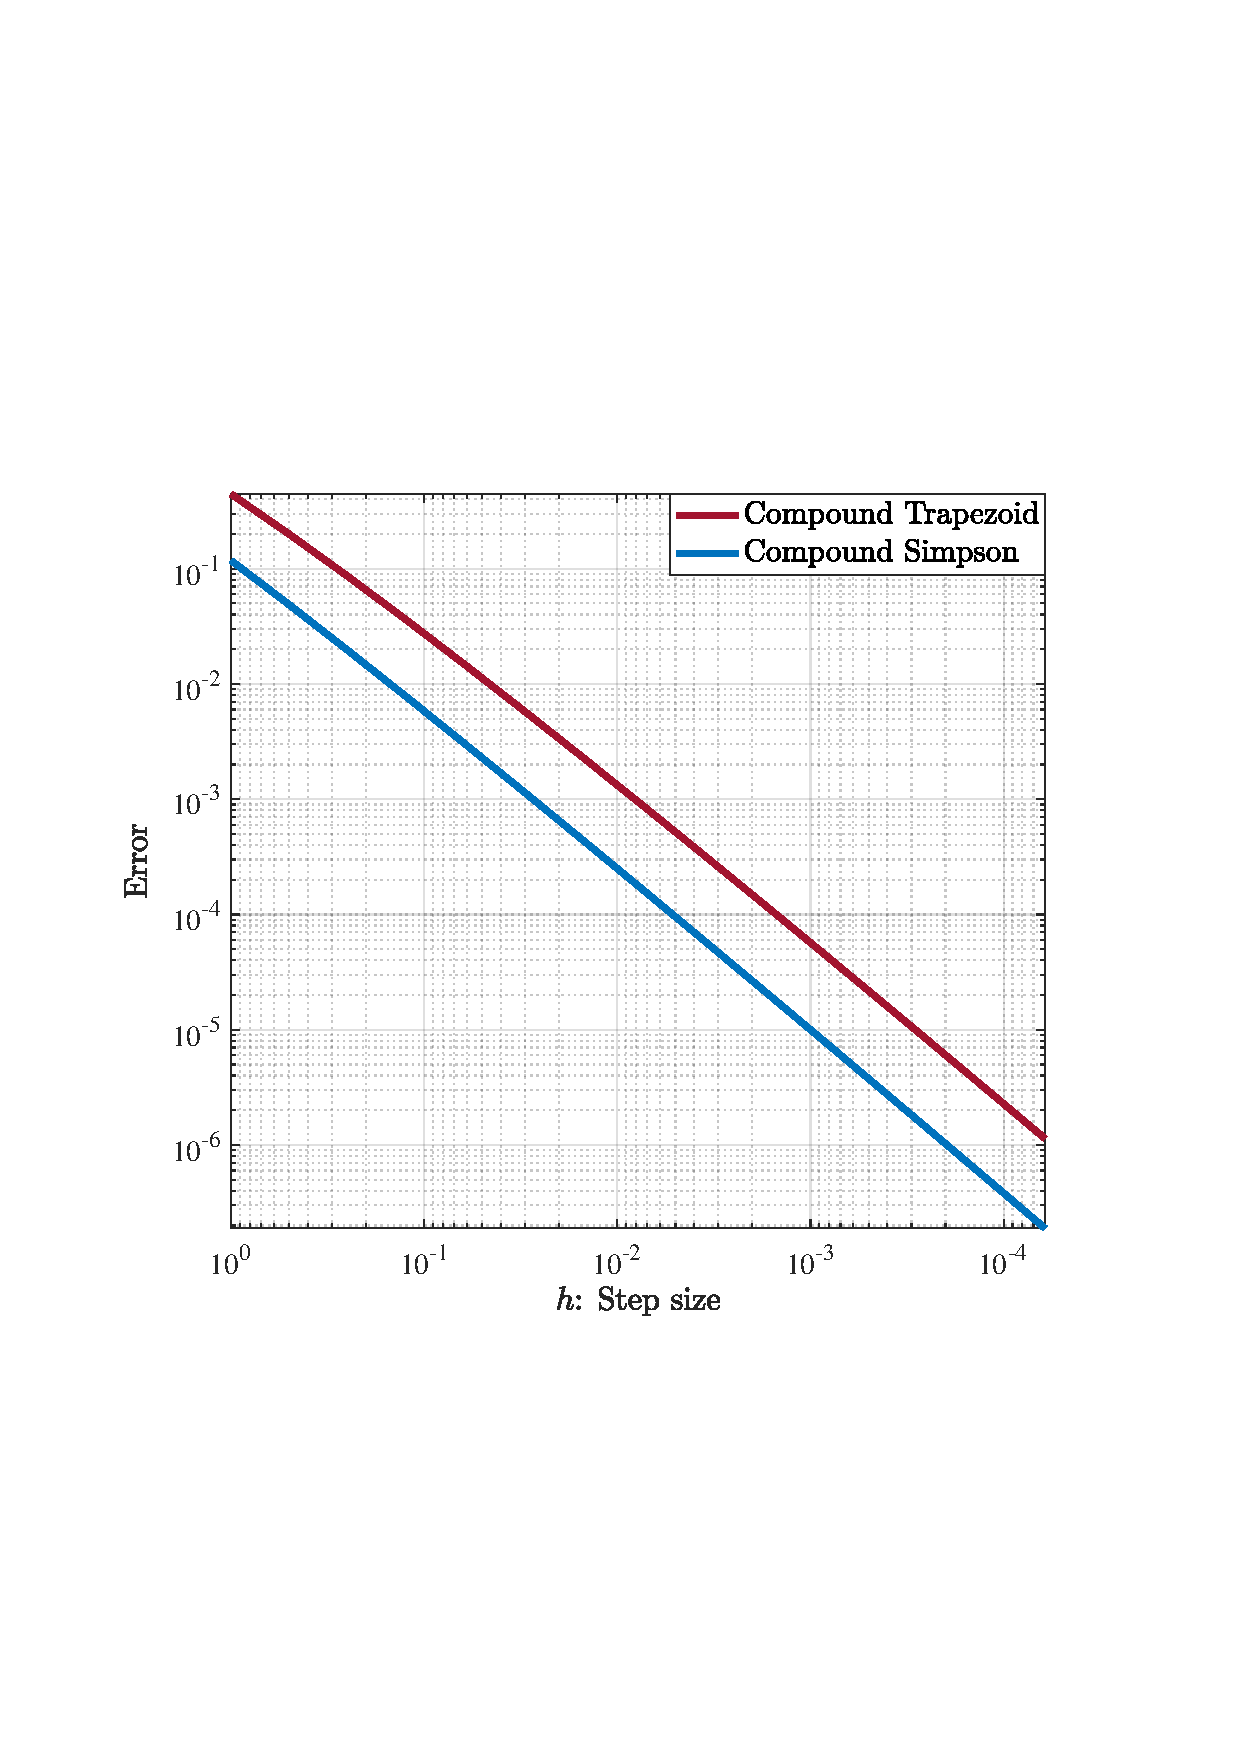
\includegraphics[width=10cm]{t_and_simpson_original.pdf} \\
    \caption{复化梯形公式和复化辛普森公式的误差随$h$变化表}
    \label{fig:t_and_simpson_R}
\end{figure}

在$h$相等的条件下,复化辛普森公式的误差约为复化梯形公式的$\frac{1}{5}$(仅从仿真结果看,不具有理论依据),说明复化辛普森公式在计算积分$\int_{0}^{1} \sqrt{x} \ln x  \ dx = -\frac{4}{9}$时精度相对更好。

\subsection*{1.4 探究:是否存在一个最小的$h$,使得精度不能再被改善?}

从表(\ref{tab:tb_t_simpson})和图(\ref{fig:t_and_simpson_R})的结果来看,随着$h$的减小,复化梯形公式和复化辛普森公式的误差均可以有效降低。所以不存在一个最小的$h$,使得精度不能再被改善。

\section*{2. 用变步长梯形公式计算积分,使其误差小于$10^{-4}$}

1.1节介绍的梯形公式可以有效提高求积精度,但是在实际计算时若精度不够可以将步长逐次分半。设将区间$[a,b]$分为$n$等份,共有$n+1$个分点,如果将求积区间再二分一次,则分店增至$2n+1$个,我们将二分前后两个积分值联系起来加以考察,注意到每个子区间$[x_k, x_{k+1}]$经过二分只增加了一个分点$x_{k+\frac{1}{2}} = \frac{1}{2}(x_k + x_{k+1})$。所以$T_{2n}$的表达式为:
\begin{equation}
    T_{2n} = \frac{h}{4} \sum_{k=0}^{n-1} [f(x_k) + f(x_{k+1})] + \frac{h}{2} \sum_{k=0}^{n-1} f(x_{k+\frac{1}{2}})
    \label{eq:step_changing_T_2n}
\end{equation}
其中$h=\frac{b-a}{n}$。由此可以得到递推公式为
\begin{equation}
    T_{2n} = \frac{1}{2} T_n + \frac{h}{2} \sum_{k=0}^{n-1} f(x_{k+\frac{1}{2}})
    \label{eq:step_changing_T_n_T_2n}
\end{equation}

仿真误差设置为$10^{-4}$,得到的仿真结果为-0.444389378040032,误差为$5.50663999154821\times10^{-5}$,此时$n=1024$,$h = 9.765625\times 10^{-4}$。此结果与表(\ref{tab:tb_t_simpson})保持一致。

\section*{3. 用Romberg公式计算积分,使其误差小于$10^{-4}$}

龙贝格求积公式也称为逐次分半加速法。是数值计算方法之一,用以求解数值积分。是在梯形公式、辛普森公式和柯特斯公式之间关系的基础上,构造出一种加速计算积分的方法。 作为一种外推算法,在不增加计算量的前提下提高了误差的精度。

设以$T_0^{(k)}$表示二分$k$次后求得的梯形值,且以$T_m^{(k)}$表示序列$\{T_0^{(k)}\}$的$m$次加速值,则递推公式可得:
\begin{equation}
    T_m^{(k)} = \frac{4^m}{4^m - 1} T_{m-1}^{(k+1)} - \frac{1}{4^m -1} T_{m-1}^{(k)}, \quad k=1,2,\cdots
    \label{eq:Romberg_T_mk}
\end{equation}

龙贝格求积算法计算过程如下:
\begin{enumerate}
    \item 取$k=0$,$h=b-a$,求$T_0^{(0)} = \frac{h}{2} [f(a) + f(b)]$。
    \item 令$1\longrightarrow k$($k$记为区间$[a,b]$的二分次数)。
    \item 求梯形值$T_0\left(\frac{b-a}{2^k}\right)$,即按递推公式(\ref{eq:step_changing_T_n_T_2n})计算$T_0^{(k)}$。
    \item 求加速值,按公式(\ref{eq:Romberg_T_mk})逐个求出T表的第$k$行其余各元素$T_j^{(k-j)}(j=1,2,\cdots,k)$。
    \item 若$|T_k^{(0)} - T_{k-1}^{(0)}|<\varepsilon $,则终止计算,并取$T_k^{(0)}\simeq I$,否则令$k+1\simeq k$转第三步继续计算。
\end{enumerate}

在仿真中,我们设置误差需低于$10^{-4}$,得到下面的Romberg算法的T表。
\begin{table}[!hpt]
    \caption{Romberg算法的T表(限于页面宽度,保留5位有效数字)}
    \label{tab:romberg_T}
    \centering
    \setlength{\tabcolsep}{1mm}{
    \begin{tabular}{cccccccccccc} \toprule
        $k$&$T_0^{(k)}$&$T_1^{(k)}$&$T_2^{(k)}$&$T_3^{(k)}$&$T_4^{(k)}$&$T_5^{(k)}$&$T_6^{(k)}$&$T_7^{(k)}$&$T_8^{(k)}$&$T_9^{(k)}$&$T_{10}^{(k)}$\\\midrule
        0 &-0.00000&&&&&&&&&& \\
        1 &-0.24506&-0.32675&&&&&&&&&\\
        2 &-0.35810&-0.36564&-0.36625&&&&&&&&\\
        3 &-0.40809&-0.41142&-0.41214&-0.41232&&&&&&&\\
        4 &-0.42947&-0.43090&-0.43120&-0.43128&-0.43130&&&&&&\\
        5 &-0.43838&-0.43898&-0.43911&-0.43914&-0.43915&-0.43915&&&&&\\
        6 &-0.44203&-0.44227&-0.44232&-0.44233&-0.44234&-0.44234&-0.44234&&&&\\
        7 &-0.44349&-0.44359&-0.44361&-0.44361&-0.44361&-0.44361&-0.44361&-0.44361&&&\\
        8 &-0.44407&-0.44411&-0.44412&-0.44412&-0.44412&-0.44412&-0.44412&-0.44412&-0.44412&&\\
        9 &-0.44430&-0.44432&-0.44431&-0.44432&-0.44432&-0.44432&-0.44432&-0.44432&-0.44432&-0.44432&\\
        10&-0.44439&-0.44440&-0.44440&-0.44440&-0.44440&-0.44440&-0.44440&-0.44440&-0.44440&-0.44440&-0.44440\\\bottomrule
    \end{tabular}}
\end{table}
% $k$&$h$&$T_0^{(k)}$&$T_1^{(k)}$&$T_2^{(k)}$&$T_3^{(k)}$&$T_4^{(k)}$&$T_5^{(k)}$&$T_6^{(k)}$&$T_7^{(k)}$&$T_8^{(k)}$&$T_9^{(k)}$&$T_{10}^{(k)}$\\\midrule
% 0 &1                       &$-2.302585\times10^{-9}$&&&&&&&&&& \\
% 1 &0.5                     &-0.245064&-0.326752&&&&&&&&&\\
% 2 &0.25                    &-0.358104&-0.365640&-0.366257&&&&&&&&\\
% 3 &0.125                   &-0.408090&-0.411422&-0.412149&-0.412329&&&&&&&\\
% 4 &$6.25\times 10^{-2}$    &-0.429474&-0.430900&-0.431209&-0.431284&-0.431302&&&&&&\\
% 5 &$3.125\times 10^{-2}$   &-0.438389&-0.438983&-0.439112&-0.439143&-0.439150&-0.439152&&&&&\\
% 6 &$1.5625\times 10^{-2}$  &-0.442030&-0.442273&-0.442325&-0.442338&-0.442341&-0.442342&-0.442342&&&&\\
% 7 &$7.8125\times 10^{-3}$  &-0.443493&-0.443591&-0.443612&-0.443617&-0.443618&-0.443618&-0.443618&-0.443618&&&\\
% 8 &$3.90625\times 10^{-3}$ &-0.444073&-0.444112&-0.444120&-0.444122&-0.444123&-0.444123&-0.444123&-0.444123&-0.444123&&\\
% 9 &$1.953125\times 10^{-3}$&-0.444301&-0.444316&-0.444319&-0.444320&-0.444320&-0.444320&-0.444320&-0.444320&-0.444320&-0.444320&\\
% 10&$9.765625\times 10^{-4}$&-0.444389&-0.444395&-0.444396&-0.444396&-0.444396&-0.444396&-0.444396&-0.444396&-0.444396&-0.444396&-0.444396\\\bottomrule

% -2.30258509299405e-09	0	0	0	0	0	0	0	0	0	0
% -0.245064539321014	-0.326752718327158	0	0	0	0	0	0	0	0	0
% -0.358104060539643	-0.365640028620885	-0.366257287514436	0	0	0	0	0	0	0	0
% -0.408090040382983	-0.411422439039205	-0.412149143966480	-0.412329112030998	0	0	0	0	0	0	0
% -0.429474585277106	-0.430900221603381	-0.431209392755193	-0.431284138828875	-0.431302667691825	0	0	0	0	0	0
% -0.438389486285633	-0.438983813019535	-0.439112123994394	-0.439143115097293	-0.439150797381035	-0.439152713896222	0	0	0	0	0
% -0.442030683768816	-0.442273430267695	-0.442325646414491	-0.442338248463197	-0.442341371760720	-0.442342150899763	-0.442342345579431	0	0	0	0
% -0.443493654984221	-0.443591186398581	-0.443612103162563	-0.443617148090987	-0.443618398237251	-0.443618710087428	-0.443618788007174	-0.443618807484437	0	0	0
% -0.444073636688462	-0.444112302135412	-0.444120573813774	-0.444122567816328	-0.444123061872755	-0.444123185111738	-0.444123215904330	-0.444123223601406	-0.444123225525608	0	0
% -0.444301037907701	-0.444316197988983	-0.444319434431103	-0.444320214276661	-0.444320407479458	-0.444320455671303	-0.444320467712477	-0.444320470722347	-0.444320471474788	-0.444320471662896	0
% -0.444389378044529	-0.444395267386984	-0.444396522456794	-0.444396824762777	-0.444396899650837	-0.444396918330244	-0.444396922997440	-0.444396924164073	-0.444396924455720	-0.444396924528632	-0.444396924546859
因为Romberg的T表中,每一列元素及对角线元素均收敛到所求的积分值$I$,所以我们将上表的第一列元素和对角线元素与准确值的误差可视化,得到图(\ref{fig:Romberg_T})。

根据T表和可视化图的显示,我们可以看到,Romberg算法可以有效收敛到准确值。在第11次递推之后,Romberg算法结果$T_{10}^{(10)}$与准确值$-\frac{4}{9}=-0.44444\cdots$的误差小于$10^{-4}$,达到预期效果,且第一列至第九列结果均收敛至准确值,验证了课本P113页结论:如果$f(x)$充分光滑,那么T表的每一列的元素及对角线元素均收敛到所求的积分值$I$,即:
\begin{equation*}
    \begin{aligned}
        & \lim_{k\rightarrow \infty} T_m^{(k)} = I \\    
        & \lim_{m\rightarrow \infty} T_m^{(0)} = I   
    \end{aligned}
\end{equation*}

\begin{figure}[t]
    \centering
    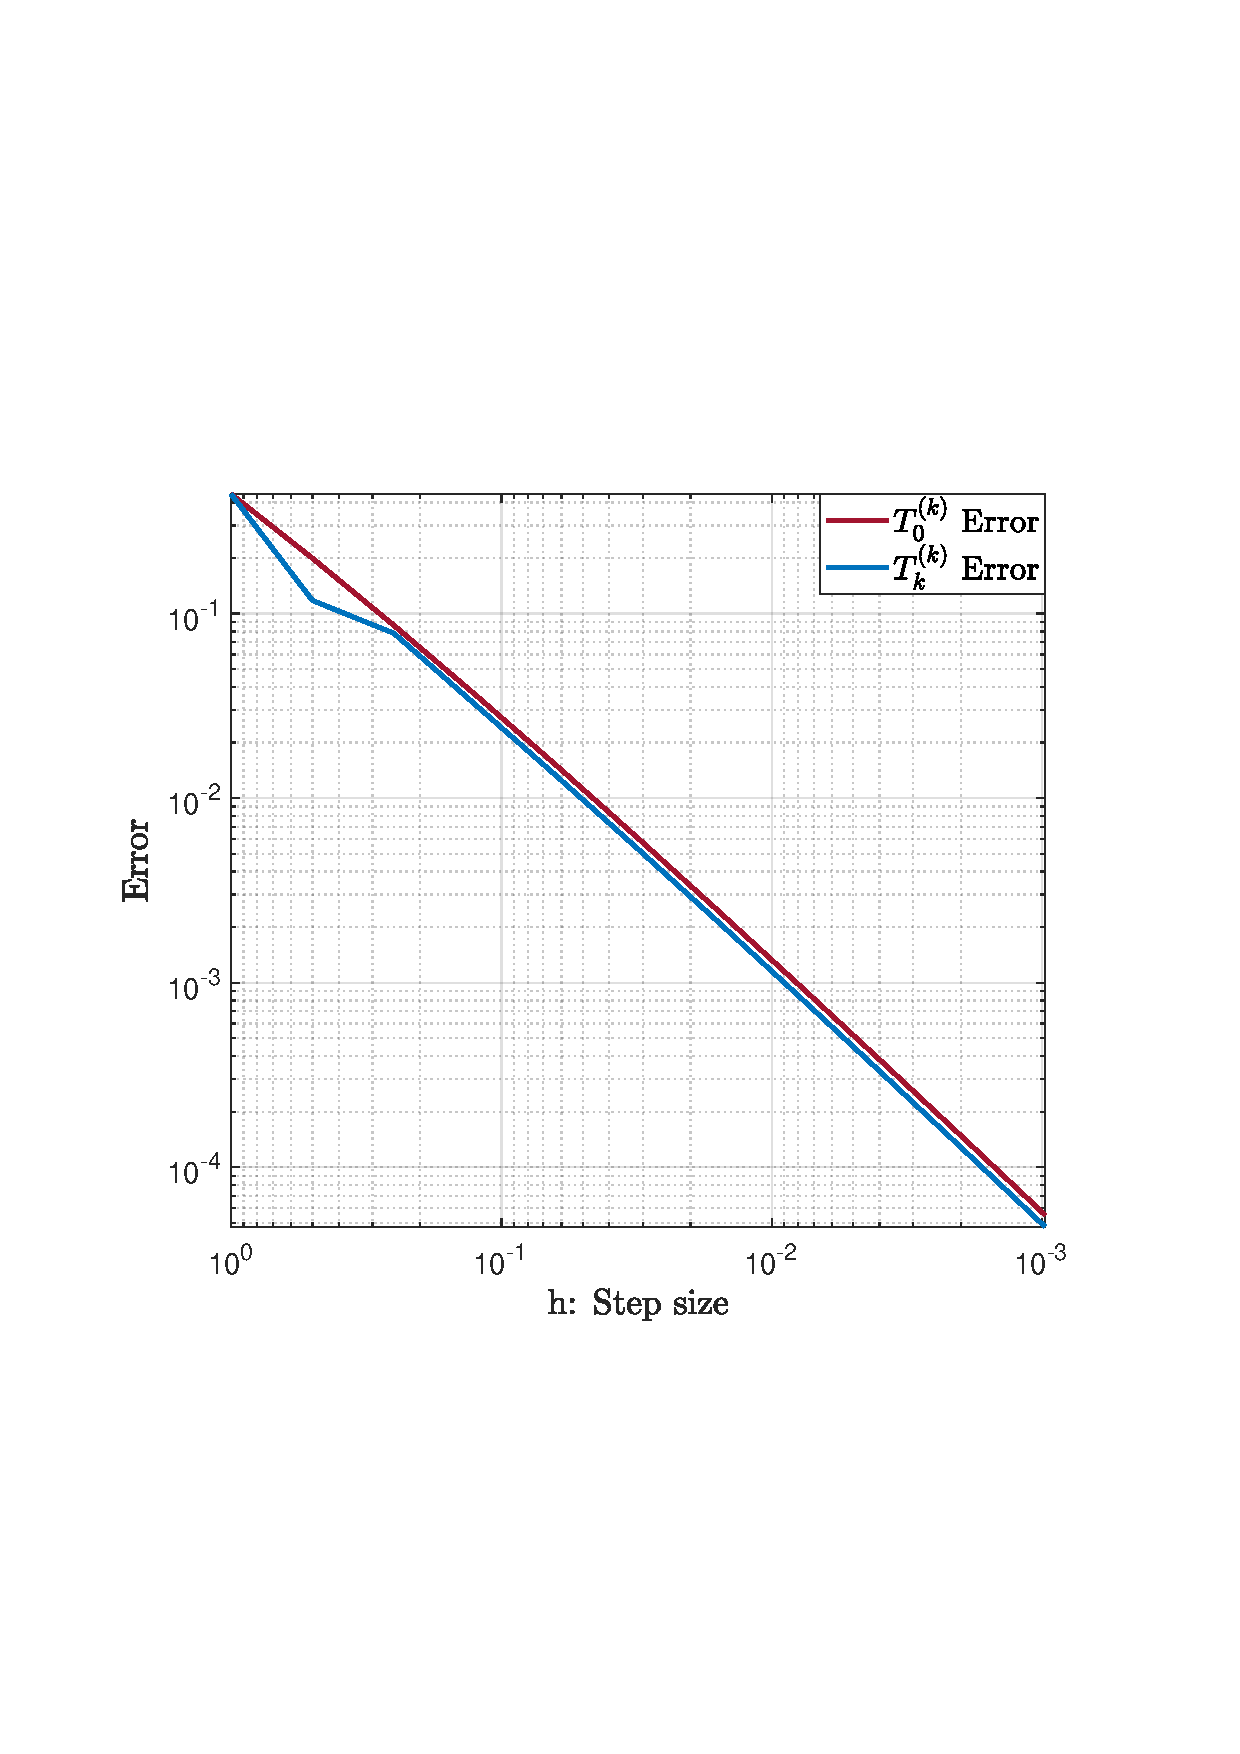
\includegraphics[width=10cm]{Romberg_1col_diag_log.pdf} \\
    \caption{Romberg算法第一列和对角线值与准确值的误差随$h$变化图}
    \label{fig:Romberg_T}
\end{figure}

\section*{4. 用自适应辛普森公式计算积分,使其误差小于$10^{-4}$}

复化求积算法通常适用于被积函数变化不太大的积分,如果在求积区间中被积函数变化很大,这时统计将区间等分,用复合求积公式计算积分工作量大,因为要达到误差要求对变化剧烈部分必须将区间细分。针对此类问题的算法技巧是在不同区间上预测被积函数变化的剧烈程度确定相应步长,这种方法称为自适应方法。自适应方法应用于复化辛普森公式中得到的称为自适应辛普森算法。

具体地,假设$S(a,b)$表示$\int_{a}^{b} f(x) \ dx = \int_{a}^{b} \sqrt{x} \ln x  \ dx$,用$I(f)$表示精确值。则自适应辛普森算法的流程如下:
\begin{enumerate}
    \item 如果$|I(f) - S(a,b) | < \varepsilon$,则算法结束;否则算法继续。
    \item 用复化辛普森公式近似计算$S(a, \frac{a+b}{2})$和$S(\frac{a+b}{2}, b)$,进行递归。
\end{enumerate}

经过仿真计算得到,自适应辛普森公式得到的计算结果为:-0.444440799763923,误差为$3.644680\times 10^{-6}$。因为自适应辛普森算法的误差是近似计算的,所以设定$\varepsilon = 10^{-4}$并不能保证一定可以搜索到误差最接近$\varepsilon$的结果,因此这里的误差要小于$10^{-4}$。

\section*{5. 比较上述5种求积公式的计算效率}

为比较5种求积公式的计算效率,我们设定相等的计算误差,即$\varepsilon < 10^{-4}$,统计五种方法达到该计算精度下的计算复杂度。计算复杂度的统计方式,按照$f(x)$参与计算的次数为量度。下面是在MATLAB程序中的复杂度统计结果:
\begin{table}[!hpt]
    \caption{5种求积公式计算复杂度统计表}
    \label{tab:Complexity}
    \centering
    \setlength{\tabcolsep}{1mm}{
    \begin{tabular}{ccccc} \toprule
        复化梯形公式&复化辛普森公式&变步长梯形公式&Romberg算法&自适应辛普森算法\\\midrule
        389      & 667        & 1024      & 512       & 147         \\\bottomrule
    \end{tabular}}
\end{table}

由上表可以得知,
\begin{enumerate}
    \item 求积效率顺序:自适应辛普森算法>复化梯形公式>Romberg算法>复化辛普森公式>变步长梯形公式。
    \item Romberg算法是基于变步长梯形公式的外推公式,有效提高收敛速率。
    \item 虽然复化梯形公式和复化辛普森公式相对复杂度较低,但是由于无法在一开始得知步长与误差的关系,所以不够灵活。
    \item 自适应辛普森算法因为可以自适应地在不同的区间上采用不同的步长,可以有效提高计算效率。
\end{enumerate}


